\documentclass{article}
\usepackage[utf8]{inputenc}
\usepackage[a4paper, total={6in, 8in}]{geometry}
\usepackage{graphicx}

\title{ECON 4P05 Assignment 1}
\author{Sannan Saleem \\}
\date{February 12, 2021}

\begin{document}

\maketitle

\newpage

\begin{center} \Huge \title{Table of Contents} \end{center}
\hspace{1.27cm}\\
\section{Introduction and Overview}
\hspace{1.27cm}Introduction to ECON 4P05 Assignment #1\\

\section{Main Results}
\subsection{ Regression vs classification; quantitative vs qualitative}
\hspace{1.27cm}Discussion of real life applications\\

\subsection{Measures of fit for linear models}
\begin{enumerate}
    \item $R^2$, Adjusted $R^2$, and SER
    \item Justification and Shortfalls
    \item Minimization/Maximization of AIC 
\end{enumerate}
\hspace{1.27cm}
\subsection{Bias-variance tradeof}
\hspace{1.27cm}Simulation Exercise 
\hspace{1.27cm}\\

\section{Bibliography}
\hspace{1.27cm} References
\hspace{1.27cm}\\

\section{Appendix}
\hspace{1.27cm} R-Studio Source Code

\newpage
\listoftables

\listoffigures


\newpage

% Introduction and Overview
\section*{1. \space Introduction and Overview}
\hspace{1.27cm}\par
ECON 4P05, taught by professor Jean Francois La-Marche, introduces the basic ideas of ”modern” statistical learning as well as predictive modeling, from a statistical, theoretical and computational perspective, along with applications in big data. With the information accumulated so far professor La-Marche, had released assignment 1 on January 29th, 2020 allowing students who had enrolled into the course, up until this point, to form groups (2 people max.) in order to further gauge their understanding of the covered material thus far. \par

This document goes on to illustrate the answers that I perceive to be "correct" in hopes to obtain partial marks that will make up a portion of the 20\% that professor La-Marche had attributed towards the final mark of any given individual student as per the course outline/syllabus. We start off by examining the difference between a regression model and a classification model in regards to the type (quantitative/qualitative) variables taken into account, discussing real life examples of where each model might prove to be useful. Furthermore, the paper moves on to describe the different measures of fit for any given linear or multiple linear regression model, finally concluding in a simulation exercise that looks at the Bias-Variance decomposition formula previously deliberated in class.\\
\hspace{1.27cm}\\
\section*{2. \space Main Results}
\subsection*{2.1 \space Regression vs. Classification; quantitative vs. qualitative}
\hspace{1.27cm}\par
When discussing the differences in a "regression" vs. that of a "classification" it is easier to think of their fundamental forms as the same. The difference lies in the output value that the regressand (dependent "Y" variable) holds. When the output variable holds a qualitative value, e.g. increase/decrease in stock price, it is referred to as a classification problem, whereas should the regressand hold a measuarble, numerical, quantitative value, it is refereed to as a regression problem.
\hspace{1.27cm}\par
\begin{enumerate}
    \item Question one asks us to examines two real life examples in which classification may be useful:\\
    \hspace{1.27cm}\\
    a) An example of a way in which classification may be useful to e-commerce business retail owners is by using machine learning and linear models such as the one below to predict customer behaviour i.e. customers can be separated into individual, pre-determined groupings based on data such as search queries, and purchasing patterns:
    \begin{equation}
    Behaviour_{i} = \beta_{0} + \beta_{1}(SQueiries_{i}) + \beta_1(purchasing_{i}) + e_{i}
    \end{equation}
    coefficients holding positive signs and any terms not already in the equation are estimated by $e_{i}$
    
   \hspace{1.27cm\\}
    b) Further more, classification models can also be used in speech prediction algotrithms to classify speech into seperate type/groups e.g. based on ethnicity by using accumulated raw data such as amplitude, wavelength, and frequency to place induvidual into groups upon matching:
    \begin{equation}
        VoiceType_{i} = \beta_{0} + \beta_{1}(Amplitude_{i}) + \beta_{2}(Wavelength_{i}) + \beta_{3}(Frequency_{i}) + e_{i}
    \end{equation}
\hspace{1.27cm}\\
\item Question two asks us to examines two real life examples in which regression may be useful:\\
    \hspace{1.27cm}\\
    a) Evaluating/predicting the price of a household (Price) for instance can be done using a regression model while taking multiple regressors such as size (size), number of rooms (rooms), and the year the house was built (year) using a multiple linear regression linear model such as:\\
    \begin{equation}
  Price_{i} = \beta_{0}(Size_{i}) + \beta_{1}(Rooms_{i}) + \beta_{2}(Year_{i}) + e_{i]}\\
   \end{equation}
   Where the Price can be measured in thousands of dollars and any unit change in the regressors will have an effect on the regressand equivalent to that of the coefficient it carries. The model such as the one illustrated above can be of use to government officials an real-estate agents alike when trying to determine the market value of a house should they need it. Of course there are a number other factors that encapsulate the value of a house at any given time which are not included in the above model but are captured by the error term "e" and the vales of $\beta_{0}, \beta_{1}, and \beta_{2}$ all hold positive values as each of the attached variable hold a positive correlation with the dependant (Y) variable.\\
   \hspace{1.27cm\\}
   b) Another example of estimating a regression could be one employed by firms to determine the wage/salary of any employee given his/her statistics and could be predicted using a regression as follows:
   
   \begin{equation}
 Salary_{i} = \beta_{0} + \beta_{1}(Age_{i}) + \beta_{2}(experience_{i}) + \beta_{3}(qualifications_{i}) + e_{i} 
   \end{equation}
   
   Where $Age_{i}$ would refer the age of an individual, experience to the number of years s/he worked, and qualifications speaking to the number of qualifications the individual had obtained, all holding positive coefficients as they are positively related to the salary/ wage an induvidual can obtain at a given moment in time. holding the same assumptions about $e_{i}$ as we did in eq. (1)
   
\end{enumerate}
\subsection*{2.2 \space Measures of Fit for Linear Models}\\
\hspace{1.27cm} When examining linear models it is useful to have a statistic that measures how well the model encapsulates the number of exogenous variables so that the researcher/reader in question can properly infer which model would be of greater use. 
\begin{enumerate}
    \item Question one examines the use of $R^2$, Adjusted $R^2$, and SER (Standard error of regression). Firstly, $R^2$ describes the level of variation in Y that can be explaind by X. Holding a value of z, where $0\leq z \leq 1$, $R^2$ can be calculated as follows:
    \hspace{1.27cm}\\
    \hspace{1.27cm}\\
    \hspace{1.27cm}\\
    \hspace{1.27cm}\\
    \begin{equation}
        R^2 = 1- \frac{\mbox{Regression Sum of Squares (RSS)}}{\mbox{TSS}}
    \end{equation}
    \hspace{1.27cm}\\
        $$\mbox{where SSR} = \Sigma (\hat{y_{i}} - \bar{y})^2 \mbox{ and TSS} = \Sigma (y_{i} - \bar{y})^2$$
    \hspace{1.27cm}\\
   $$ R^2 = \frac{\Sigma (\hat{y_{i}} - \bar{y})^2}{\Sigma (y_{i} - \bar{y})^2}= 1- \sum \frac{\hat{u_{i}}^2}{({y_{i} -\bar{y}_{i})^2}}$$
   
   Secondly, adjusted $R^2$ is a slightly differed version of $R^2$ which has been adjusted to the number of predictors in the model so that the adjusted $R^2$ only increases if the addition of a new variable causes an improvement in the model.
   \begin{equation}
  \bar{R}^2 = 1- \frac{\hat{u_{i}}^2/ (N - K - 1)}{({y_{i}-\bar{y}_{i})^2}/(N-1))} = 1- \frac{SSR/(N-K-1)}{TSS/(N-1)}
   \end{equation}
   Finally, taking a look at SER (Standard error of Regression), SER measures how far the observed values fall from the regression line i.e. the distribution spread of u.
   \begin{equation}
    SER = \sqrt{\frac{1}{n-2} \sum_{i=1}^{n}\hat{u_{i}}^2}
    \end{equation}
    
    \item Given $y_{i} = x_{i}\Beta +e_{i}$ and assuming that the error term is standard normal, the optimization problem follows as:
    \begin{equation}
     \max_{\beta ,\sigma^2}\ln L(\beta ,\sigma^2)= - \frac{n}{2}\ln(2\pi)-\frac{n}{2}\ln\sigma^2 - \frac{\sum^n_{i=1}(y_i - x_i\beta)^2} {2\sigma^2} 
    \end{equation}
   then differentiating $-\sum \frac{(y_{i}-x_{i}\beta)^2}{2\theta^2}$ with respect to $\beta$ and setting it equal to zero yeilds $-\sum \frac{(y_{i}-x_{i}^\beta)x_{i}}{\theta^2}$ and so:

    \begin{equation}
    \hat{\beta }=\frac{\sum x_iy_i}{\sum x_i^2}  \\
    \end{equation}
Moreover, if $-\sum \frac{(y_{i}-x_{i}\beta)^2}{2\theta^2}$ is differentiated with respect to $\theta^2$ and then set to zero, upon solving the set for $\theta^2$ yeilds $\frac{-n}{2\theta^2}+\frac{\sum (y_{i}-x_{i}^\beta)}{2\theta^2}=0$, therefore it can be concluded that:
    \begin{equation}
    \hat{\sigma }^2=\frac{\sum (y_i-x_i^\beta )^2}{n} \\
        \end{equation}
        \hspace{1.27cm}\\
        \item Penalizeing models with a large number of parameters leads to various criterion functions that can be used to rank competing models.The most widely used of these is probably the Akaike information criterion, or AIC.
        \begin{equation}
            AIC = \^{l} - p
        \end{equation} considering AIC to fit a model, if the the number of parameters are increased, the log likelihood will also be improved, but may lead to a shortfall that is "over-fitting" the model. The AIC penalizes for increasing the number of parameters, therefore minimizing the AIC allows for the selection of a model where the improvement in log likelihood outweighs the penalty for increasing the number of parameters.
    
\end{enumerate}
\newpage
\subsection*{2.3 \space Bias-Variance trade off}
The bias-variance decomposition formula was previously derived.This simulations exercise illustrates one of the three components of the decomposition. Assuming that the systematic part of the model looks like:
\begin{equation}
    f(x) = 0.5x + \sqrt{max(x,0)} - cos(x) + 2
\end{equation}
while the error term follows the standard normal distribution, and assume that x is uniformly distributed in the interval -3 to +3. 1000 observations on the output variable can then be generated as $y = f(x) + e$.
% latex table generated in R 4.0.2 by xtable 1.8-4 package
% Fri Feb 12 12:04:57 2021
\begin{table}[ht]
\caption{20 Observations of 5 induvidual samples}
\centering
\begin{tabular}{rrrrrrrrrrr}
  \hline
 Observation \# & x_{1} & y_{1} & x_{2} & y_{2} & x_{3} & y_{3} & x_{4} & y_{4} & x_{5} & y_{5} \\ 
  \hline
975 & -2.11 & -0.48 & -0.40 & 1.00 & -2.09 & 0.75 & 2.51 & 5.50 & 0.71 & 1.88 \\ 
  844 & 0.61 & 2.65 & -2.08 & 1.76 & 1.10 & 3.35 & 1.00 & 3.55 & -2.54 & 2.31 \\ 
  896 & 1.75 & 4.27 & 0.61 & 1.35 & 0.54 & 2.05 & -2.18 & 1.08 & 2.52 & 5.63 \\ 
  577 & -1.00 & 0.46 & 1.38 & 4.27 & 2.23 & 4.90 & -2.32 & 2.50 & -0.76 & 0.88 \\ 
  614 & -0.88 & 3.03 & 1.57 & 4.93 & 0.09 & 1.14 & -2.79 & 2.32 & 1.94 & 6.12 \\ 
  325 & 2.10 & 4.51 & -1.63 & 1.34 & -2.19 & 1.87 & -1.00 & 0.46 & 0.61 & 2.61 \\ 
  269 & 2.16 & 4.93 & -0.21 & 2.31 & 1.33 & 2.04 & 1.94 & 6.12 & 0.71 & 3.87 \\ 
  695 & 0.35 & 0.20 & 2.63 & 6.38 & -1.60 & 2.00 & -0.21 & 1.90 & 1.62 & 3.78 \\ 
  137 & -2.59 & 2.05 & 2.84 & 5.75 & 1.33 & 5.05 & 0.99 & 2.73 & 2.39 & 5.39 \\ 
  659 & 0.95 & 3.09 & -2.59 & 1.54 & 1.08 & 3.22 & -2.58 & 0.17 & -1.30 & 0.71 \\ 
  386 & 2.14 & 6.56 & 2.02 & 4.15 & -1.36 & 0.52 & -1.44 & 1.14 & 2.90 & 5.52 \\ 
  595 & -1.03 & -0.10 & 2.29 & 6.57 & 2.39 & 5.39 & 0.45 & 1.59 & 1.33 & 4.68 \\ 
  767 & 0.78 & 1.54 & 0.49 & 2.65 & 1.28 & 3.84 & 0.70 & 3.16 & -0.29 & 1.03 \\ 
  310 & -2.80 & 2.94 & -0.80 & 0.00 & 0.64 & 2.45 & -0.70 & -0.40 & 2.47 & 3.72 \\ 
  981 & 1.43 & 1.97 & 2.52 & 5.63 & 0.45 & 3.34 & 2.06 & 4.73 & 1.88 & 3.71 \\ 
  47 & 2.17 & 4.72 & 2.06 & 4.10 & 2.85 & 5.27 & 0.50 & 0.60 & 0.66 & 2.29 \\ 
  400 & -1.99 & 0.42 & 0.54 & 2.05 & 1.16 & 3.77 & -1.00 & 1.89 & 1.57 & 2.17 \\ 
  193 & -1.87 & 1.33 & 2.05 & 6.37 & 1.38 & 3.36 & 2.93 & 8.05 & 2.99 & 5.72 \\ 
  621 & -0.06 & 1.82 & -2.19 & 0.14 & -2.59 & 2.05 & -0.98 & 0.88 & -1.80 & 1.86 \\ 
  312 & 0.29 & -0.28 & 2.54 & 6.77 & -0.88 & 1.08 & -1.57 & -0.08 & 2.26 & 5.94 \\ 
   \hline
\end{tabular}
\end{table}\\
Table 1 above represents the 20 different observations of each sample where the ordered pair $(x_{n},y_{n})$ belongs to the n^th sample set.
\newpage
% Table created by stargazer v.5.2.2 by Marek Hlavac, Harvard University. E-mail: hlavac at fas.harvard.edu
% Date and time: Fri, Feb 12, 2021 - 12:10:40
\begin{table}[!htbp] \centering 
  \caption{Sample 1 Regression Results} 
  \label{} 
\begin{tabular}{@{\extracolsep{5pt}}lcc} 
\\[-1.8ex]\hline 
\hline \\[-1.8ex] 
 & \multicolumn{2}{c}{\textit{Dependent variable:}} \\ 
\cline{2-3} 
\\[-1.8ex] & \multicolumn{2}{c}{y} \\ 
\\[-1.8ex] & (1) & (2)\\ 
\hline \\[-1.8ex] 
 x & 0.739$^{***}$ & $-$0.029 \\ 
  & (0.213) & (0.711) \\ 
  & & \\ 
 I(x$\hat{\mkern6mu}$2) &  & 0.361 \\ 
  &  & (0.614) \\ 
  & & \\ 
 I(x$\hat{\mkern6mu}$3) &  & 0.521 \\ 
  &  & (0.400) \\ 
  & & \\ 
 I(x$\hat{\mkern6mu}$4) &  & 0.0002 \\ 
  &  & (0.119) \\ 
  & & \\ 
 I(x$\hat{\mkern6mu}$5) &  & $-$0.060 \\ 
  &  & (0.057) \\ 
  & & \\ 
 Constant & 2.267$^{***}$ & 1.170$^{**}$ \\ 
  & (0.353) & (0.531) \\ 
  & & \\ 
\hline \\[-1.8ex] 
Observations & 20 & 20 \\ 
R$^{2}$ & 0.400 & 0.763 \\ 
Adjusted R$^{2}$ & 0.367 & 0.679 \\ 
Residual Std. Error & 1.579 (df = 18) & 1.125 (df = 14) \\ 
F Statistic & 12.023$^{***}$ (df = 1; 18) & 9.024$^{***}$ (df = 5; 14) \\ 
\hline 
\hline \\[-1.8ex] 
\textit{Note:}  & \multicolumn{2}{r}{$^{*}$p$<$0.1; $^{**}$p$<$0.05; $^{***}$p$<$0.01} \\ 
\end{tabular} 
\end{table} 
\hspace{1.27cm} \par
Taking a look at sample 1 regression results above, its clear to see that after comparing values of $\bar{R^2}$ between the linear(1) and linear+ (2) model, the data comprising of the model with polynomial to degree 5 has an over ll better fit (0.679 vs. 0.367). This implies that approx. 67.9\% of variation in Y can be explained by the independent variables when contrasted with the linear model in which only 36.7\% of the variation in Y can be explained by the independent variable X
\newpage 
% Table created by stargazer v.5.2.2 by Marek Hlavac, Harvard University. E-mail: hlavac at fas.harvard.edu
% Date and time: Fri, Feb 12, 2021 - 12:12:19
\begin{table}[!htbp] \centering 
  \caption{Sample 2 Regression Results} 
  \label{} 
\begin{tabular}{@{\extracolsep{5pt}}lcc} 
\\[-1.8ex]\hline 
\hline \\[-1.8ex] 
 & \multicolumn{2}{c}{\textit{Dependent variable:}} \\ 
\cline{2-3} 
\\[-1.8ex] & \multicolumn{2}{c}{y} \\ 
\\[-1.8ex] & (1) & (2)\\ 
\hline \\[-1.8ex] 
 x & 1.120$^{***}$ & 1.045 \\ 
  & (0.146) & (0.626) \\ 
  & & \\ 
 I(x$\hat{\mkern6mu}$2) &  & 0.535 \\ 
  &  & (0.313) \\ 
  & & \\ 
 I(x$\hat{\mkern6mu}$3) &  & 0.051 \\ 
  &  & (0.273) \\ 
  & & \\ 
 I(x$\hat{\mkern6mu}$4) &  & $-$0.029 \\ 
  &  & (0.046) \\ 
  & & \\ 
 I(x$\hat{\mkern6mu}$5) &  & $-$0.011 \\ 
  &  & (0.029) \\ 
  & & \\ 
 Constant & 2.689$^{***}$ & 1.472$^{***}$ \\ 
  & (0.274) & (0.411) \\ 
  & & \\ 
\hline \\[-1.8ex] 
Observations & 20 & 20 \\ 
R$^{2}$ & 0.765 & 0.891 \\ 
Adjusted R$^{2}$ & 0.752 & 0.852 \\ 
Residual Std. Error & 1.142 (df = 18) & 0.881 (df = 14) \\ 
F Statistic & 58.607$^{***}$ (df = 1; 18) & 22.926$^{***}$ (df = 5; 14) \\ 
\hline 
\hline \\[-1.8ex] 
\textit{Note:}  & \multicolumn{2}{r}{$^{*}$p$<$0.1; $^{**}$p$<$0.05; $^{***}$p$<$0.01} \\ 
\end{tabular} 
\end{table} 
\hspace{1.27cm} \par
Taking a look at sample 2 regression results above, its clear to see that after comparing values of $\bar{R^2}$ between the linear(1) and linear+ (2) model, the data comprising of the model with polynomial to degree 5 has an over ll better fit (0.852 vs. 0.752). This implies that approx. 85.2\% of variation in Y can be explained by the independent variables when contrasted with the linear model in which only 75.2\% of the variation in Y can be explained by the independent variable X
\newpage

% Table created by stargazer v.5.2.2 by Marek Hlavac, Harvard University. E-mail: hlavac at fas.harvard.edu
% Date and time: Fri, Feb 12, 2021 - 12:12:46
\begin{table}[!htbp] \centering 
  \caption{Sample 3 Regression Results} 
  \label{} 
\begin{tabular}{@{\extracolsep{5pt}}lcc} 
\\[-1.8ex]\hline 
\hline \\[-1.8ex] 
 & \multicolumn{2}{c}{\textit{Dependent variable:}} \\ 
\cline{2-3} 
\\[-1.8ex] & \multicolumn{2}{c}{y} \\ 
\\[-1.8ex] & (1) & (2)\\ 
\hline \\[-1.8ex] 
 x & 0.761$^{***}$ & 1.134$^{**}$ \\ 
  & (0.132) & (0.479) \\ 
  & & \\ 
 I(x$\hat{\mkern6mu}$2) &  & 0.429 \\ 
  &  & (0.314) \\ 
  & & \\ 
 I(x$\hat{\mkern6mu}$3) &  & $-$0.074 \\ 
  &  & (0.242) \\ 
  & & \\ 
 I(x$\hat{\mkern6mu}$4) &  & $-$0.020 \\ 
  &  & (0.043) \\ 
  & & \\ 
 I(x$\hat{\mkern6mu}$5) &  & $-$0.0001 \\ 
  &  & (0.027) \\ 
  & & \\ 
 Constant & 2.599$^{***}$ & 1.665$^{***}$ \\ 
  & (0.212) & (0.429) \\ 
  & & \\ 
\hline \\[-1.8ex] 
Observations & 20 & 20 \\ 
R$^{2}$ & 0.649 & 0.808 \\ 
Adjusted R$^{2}$ & 0.629 & 0.740 \\ 
Residual Std. Error & 0.924 (df = 18) & 0.773 (df = 14) \\ 
F Statistic & 33.222$^{***}$ (df = 1; 18) & 11.819$^{***}$ (df = 5; 14) \\ 
\hline 
\hline \\[-1.8ex] 
\textit{Note:}  & \multicolumn{2}{r}{$^{*}$p$<$0.1; $^{**}$p$<$0.05; $^{***}$p$<$0.01} \\ 
\end{tabular} 
\end{table} 
\hspace{1.27cm} \par
Taking a look at sample 3 regression results above, its clear to see that after comparing values of $\bar{R^2}$ between the linear(1) and linear+ (2) model, the data comprising of the model with polynomial to degree 5 has an over ll better fit (0.740 vs. 0.629). This implies that approx. 74.0\% of variation in Y can be explained by the independent variables when contrasted with the linear model in which only 62.9\% of the variation in Y can be explained by the independent variable X
\newpage

% Table created by stargazer v.5.2.2 by Marek Hlavac, Harvard University. E-mail: hlavac at fas.harvard.edu
% Date and time: Fri, Feb 12, 2021 - 12:13:09
\begin{table}[!htbp] \centering 
  \caption{Sample 4 Regression Results} 
  \label{} 
\begin{tabular}{@{\extracolsep{5pt}}lcc} 
\\[-1.8ex]\hline 
\hline \\[-1.8ex] 
 & \multicolumn{2}{c}{\textit{Dependent variable:}} \\ 
\cline{2-3} 
\\[-1.8ex] & \multicolumn{2}{c}{y} \\ 
\\[-1.8ex] & (1) & (2)\\ 
\hline \\[-1.8ex] 
 x & 0.994$^{***}$ & 1.332$^{**}$ \\ 
  & (0.192) & (0.601) \\ 
  & & \\ 
 I(x$\hat{\mkern6mu}$2) &  & 0.581 \\ 
  &  & (0.464) \\ 
  & & \\ 
 I(x$\hat{\mkern6mu}$3) &  & $-$0.214 \\ 
  &  & (0.291) \\ 
  & & \\ 
 I(x$\hat{\mkern6mu}$4) &  & $-$0.034 \\ 
  &  & (0.066) \\ 
  & & \\ 
 I(x$\hat{\mkern6mu}$5) &  & 0.015 \\ 
  &  & (0.032) \\ 
  & & \\ 
 Constant & 2.579$^{***}$ & 1.461$^{**}$ \\ 
  & (0.329) & (0.546) \\ 
  & & \\ 
\hline \\[-1.8ex] 
Observations & 20 & 20 \\ 
R$^{2}$ & 0.597 & 0.787 \\ 
Adjusted R$^{2}$ & 0.575 & 0.710 \\ 
Residual Std. Error & 1.462 (df = 18) & 0.981 (df = 14) \\ 
F Statistic & 26.708$^{***}$ (df = 1; 18) & 10.316$^{***}$ (df = 5; 14) \\ 
\hline 
\hline \\[-1.8ex] 
\textit{Note:}  & \multicolumn{2}{r}{$^{*}$p$<$0.1; $^{**}$p$<$0.05; $^{***}$p$<$0.01} \\ 
\end{tabular} 
\end{table} 
\hspace{1.27cm} \par
Taking a look at sample 1 regression results above, its clear to see that after comparing values of $\bar{R^2}$ between the linear(1) and linear+ (2) model, the data comprising of the model with polynomial to degree 5 has an over ll better fit (0.710 vs. 0.575). This implies that approx. 71.0\% of variation in Y can be explained by the independent variables when contrasted with the linear model in which only 57.5\% of the variation in Y can be explained by the independent variable X
\newpage

% Table created by stargazer v.5.2.2 by Marek Hlavac, Harvard University. E-mail: hlavac at fas.harvard.edu
% Date and time: Fri, Feb 12, 2021 - 12:13:34
\begin{table}[!htbp] \centering 
  \caption{Sample 5 Regression Results} 
  \label{} 
\begin{tabular}{@{\extracolsep{5pt}}lcc} 
\\[-1.8ex]\hline 
\hline \\[-1.8ex] 
 & \multicolumn{2}{c}{\textit{Dependent variable:}} \\ 
\cline{2-3} 
\\[-1.8ex] & \multicolumn{2}{c}{y} \\ 
\\[-1.8ex] & (1) & (2)\\ 
\hline \\[-1.8ex] 
 x & 0.902$^{***}$ & 1.332$^{**}$ \\ 
  & (0.163) & (0.601) \\ 
  & & \\ 
 I(x$\hat{\mkern6mu}$2) &  & 0.581 \\ 
  &  & (0.464) \\ 
  & & \\ 
 I(x$\hat{\mkern6mu}$3) &  & $-$0.214 \\ 
  &  & (0.291) \\ 
  & & \\ 
 I(x$\hat{\mkern6mu}$4) &  & $-$0.034 \\ 
  &  & (0.066) \\ 
  & & \\ 
 I(x$\hat{\mkern6mu}$5) &  & 0.015 \\ 
  &  & (0.032) \\ 
  & & \\ 
 Constant & 2.596$^{***}$ & 1.461$^{**}$ \\ 
  & (0.302) & (0.546) \\ 
  & & \\ 
\hline \\[-1.8ex] 
Observations & 20 & 20 \\ 
R$^{2}$ & 0.630 & 0.787 \\ 
Adjusted R$^{2}$ & 0.609 & 0.710 \\ 
Residual Std. Error & 1.139 (df = 18) & 0.981 (df = 14) \\ 
F Statistic & 30.635$^{***}$ (df = 1; 18) & 10.316$^{***}$ (df = 5; 14) \\ 
\hline 
\hline \\[-1.8ex] 
\textit{Note:}  & \multicolumn{2}{r}{$^{*}$p$<$0.1; $^{**}$p$<$0.05; $^{***}$p$<$0.01} \\ 
\end{tabular} 
\end{table} 
\hspace{1.27cm} \par
Taking a look at sample 1 regression results above, its clear to see that after comparing values of $\bar{R^2}$ between the linear(1) and linear+ (2) model, the data comprising of the model with polynomial to degree 5 has an over ll better fit (0.710 vs. 0.609). This implies that approx. 71.0\% of variation in Y can be explained by the independent variables when contrasted with the linear model in which only 60.9\% of the variation in Y can be explained by the independent variable X
\newpage

\begin{figure}[!htb]
\caption{Simple x/y scatter plot containing all 1000 observations w/ fitted linear regression line}
\label{Figure 1}
\begin{center}
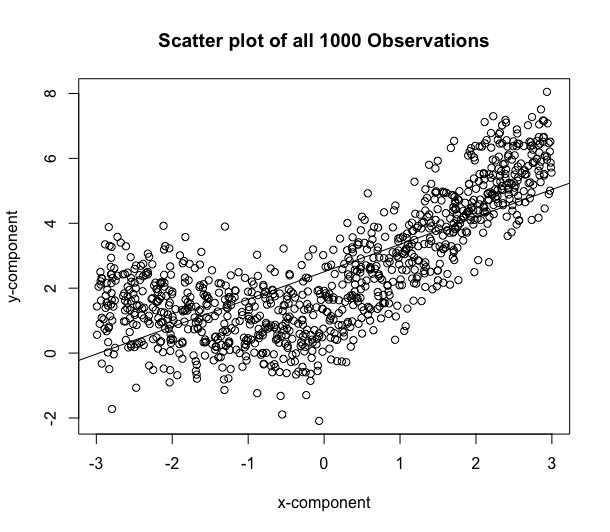
\includegraphics[scale=0.8]{sample_1k.png}
\end{center}
\end{figure}
The volatility of the scatter plot seems quite consistent when comapring the plotted points tot he regression line, the scatter plot also indicates a positive linear relationship between x and y.


\newpage

\begin{figure}[!htb]
\caption{Sample 1 Scatter plot with fitted line for linear/linear+ models}
\label{returns_microsoft}
\begin{center}
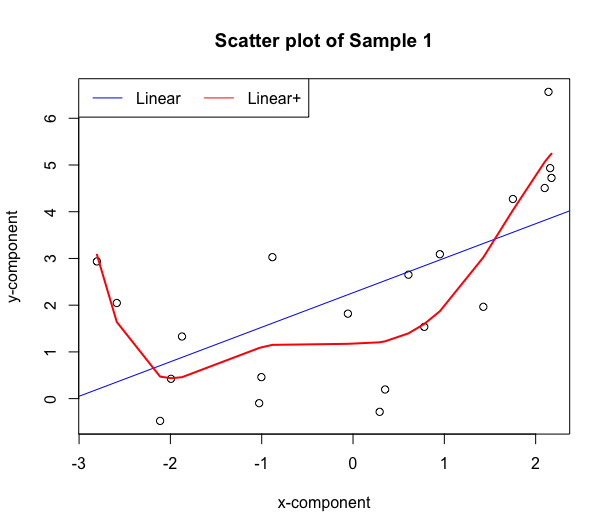
\includegraphics[scale = 0.8]{sample1.png}
\end{center}
\end{figure}
The Linear+ fitted line seems to better encapsulate the data trend of Sample 1 as it is less volatile when comparing the plotted points to the linear fitted regression line. The relationship between x and y is unclear but indicates a somewhat positive relationship.
\newpage

\begin{figure}[!htb]
\caption{Sample 2 Scatter plot with fitted line for linear/linear+ models}
\label{returns_microsoft}
\begin{center}
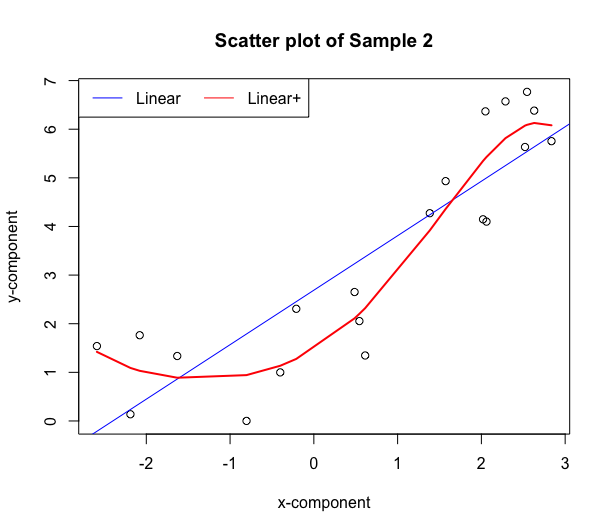
\includegraphics[scale=0.8]{sample2.png}
\end{center}
\end{figure}
The Linear+ fitted line seems to better encapsulate the data trend of Sample 2 as it is less volatile when comparing the plotted points to the linear fitted regression line. The relationship between x and y indicates a positive almost exponential like relationship.
\newpage

\begin{figure}[!htb]
\caption{Sample 3 Scatter plot with fitted line for linear/linear+ models}
\label{returns_microsoft}
\begin{center}
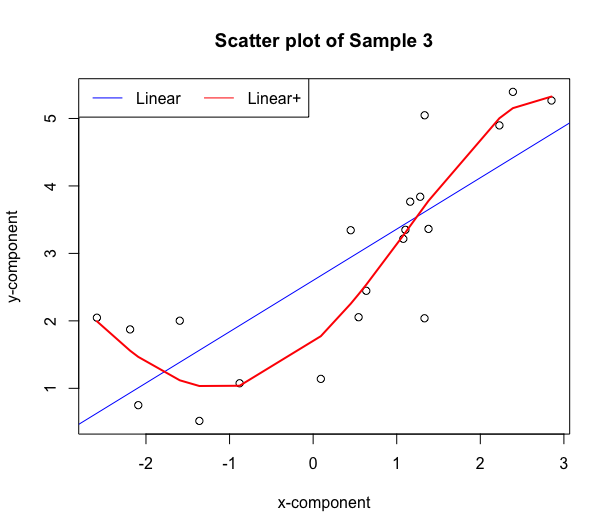
\includegraphics[scale=0.8]{sample3.png}
\end{center}
\end{figure}
The Linear+ fitted line seems to better encapsulate the data trend of Sample 3 as it is less volatile when comparing the plotted points to the linear fitted regression line. The relationship between x and y indicates a positive relationship where the y component increases as the x-compents increases.
\newpage

\begin{figure}[!htb]
\caption{Sample 4 Scatter plot with fitted line for linear/linear+ models}
\label{returns_microsoft}
\begin{center}
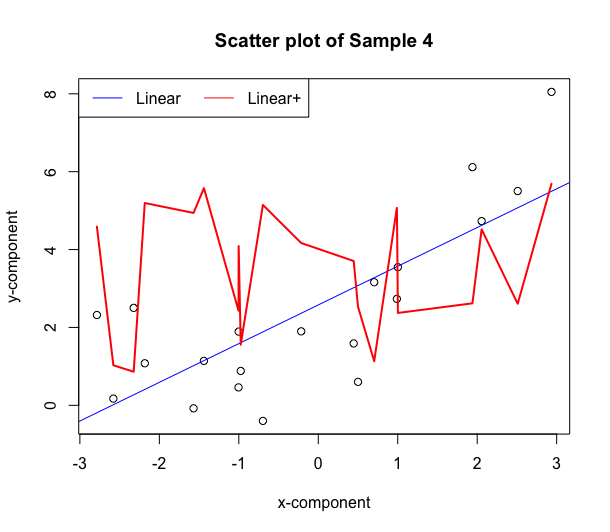
\includegraphics[scale=0.8]{sample4.png}
\end{center}
\end{figure}
The Linear fitted line seems to better encapsulate the data trend of Sample 4 at first glance before examining the quantitative regression results, when comparing the plotted points to the linear+ fitted regression line. Upon further examination of Table(5) it is clearer to see that the Linear+ regression line is a better fit for the data, once again, the relationship between x and y indicates a somewhat positive relationship.
\newpage

\begin{figure}[!htb]
\caption{Sample 5 Scatter plot with fitted line for linear/linear+ models}
\label{returns_microsoft}
\begin{center}
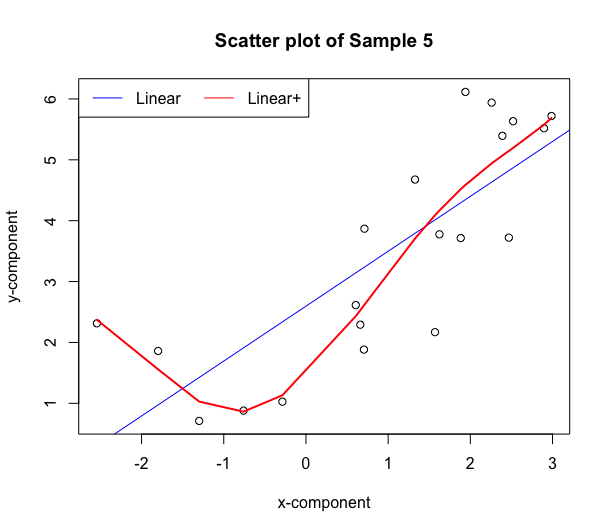
\includegraphics[scale=0.8]{sample5.png}
\end{center}
\end{figure}
The Linear+ fitted line seems to far better encapsulate the data trend of Sample 5 as it is much less volatile when comparing the plotted points to the linear+ fitted regression line, passing through some points and close enough others to represent lack of volatility. The relationship between x and y indicates a somewhat positive relationship.
\newpage
\section*{3. \space Bibliography}
\begin{thebibliography}{9}
\bibitem{latexcompanion} 
Gareth James, Daniela Witten, Trevor Hastie, and Robert Tibshirani. 
\textit{An Introduction to Statistical Learning with Applications in R (2017)}. 
New York, N.Y:Springer. Pages (29-33;33-37)

\bibitem{latexcompanion} 
Oestrich, M. (2020) 
\textit{ECON 3P90 - Lab 9. https://lms.brocku.ca/access/content/group/ae6a45db-69ba-45d2-82fb-9c979d6c7d01/Lab/Lab%209%20-%20Binary%20Variables%2C%20Part%20II.pdf}. 
Brock University, St. Catherines, ON}

\bibitem{latexcompanion} 
Oestrich, M. (2020) 
\textit{ECON 3P90 - Lab 5. https://lms.brocku.ca/access/content/group/ae6a45db-69ba-45d2-82fb-9c979d6c7d01/Lab/Lab%205%20-%20Nonlinear%20Regression.pdf}. 
Brock University, St. Catherines, ON}
\end{thebibliography}

\newpage
\section{4. \space Appendix}
\subsection*{R-Studio Source Code:}
\begin{verbatim}
    #given
set.seed(19)
nobs<-1000
sigma<-1
x_max<-3
x_test<-3.2
x<-x_max*(2*runif(nobs)-1)
e<-sigma*rnorm(nobs)
f<-0.5*x + sqrt(pmax(x,0)) - cos(x) +2
y<-f+e

#------------------------part (a)------------------------------

#create a scatterplot
plot(x,y, abline(lm(y~x)), 
     main = "Scatter plot of all 1000 Observations",
     xlab = "x-component", ylab = "y-component")

#------------------------part (b)------------------------------

#create a dataframe for all 1000 values of "x" and "y
newdat <- data.frame(x = x, y = y)

#draw 5 samples (20 obs./sample) from data frame created 
sample_1 <- newdat[sample(nrow(newdat), 20),]
sample_2 <- newdat[sample(nrow(newdat), 20),]
sample_3 <- newdat[sample(nrow(newdat), 20),]
sample_4 <- newdat[sample(nrow(newdat), 20),]
sample_5 <- newdat[sample(nrow(newdat), 20),]

#------------------------part (c)---------------------------------
#work on sample 1 to create lm/lm with a polynomial of order 5 in x
lm_1 <- lm(formula = y ~ x ,
                  data = sample_1)
summary(lm_1)

lm_2 <- lm(formula = y ~ x + I(x^2) + I(x^3) + I(x^4) + I(x^5) ,
           data = sample_1)
summary(lm_2)

lm_3 <- lm(formula = y ~ x ,
           data = sample_2)
summary(lm_3)

lm_4 <- lm(formula = y ~ x + I(x^2) + I(x^3) + I(x^4) + I(x^5) ,
           data = sample_2)
summary(lm_4)

lm_5 <- lm(formula = y ~ x ,
           data = sample_3)
summary(lm_5)

lm_6 <- lm(formula = y ~ x + I(x^2) + I(x^3) + I(x^4) + I(x^5) ,
           data = sample_3)
summary(lm_6)

lm_7 <- lm(formula = y ~ x ,
           data = sample_4)
summary(lm_7)

lm_8 <- lm(formula = y ~ x + I(x^2) + I(x^3) + I(x^4) + I(x^5) ,
           data = sample_5)
summary(lm_8)

lm_9 <- lm(formula = y ~ x ,
           data = sample_5)
summary(lm_9)

lm_10 <- lm(formula = y ~ x + I(x^2) + I(x^3) + I(x^4) + I(x^5) ,
           data = sample_5)
summary(lm_10)

#-------------------------Part(d)--------------------------------------------
#scatterplots with fitted lines sample 1
plot(sample_1,
     main = "Scatter plot of Sample 1",
     xlab = "x-component", ylab = "y-component")

abline(lm_1, col = "blue")

order_id_1 <- order(sample_1$x)

lines(sample_1$x[order_id_1],
      fitted(lm_2)[order_id_1],
      col = "red", lwd = 2)

legend("topleft", horiz = TRUE,
       legend = c("Linear", "Linear+"), col = c("blue", "red"),
       lty = c(1, 1))

#scatterplots with fitted lines sample 2
plot(sample_2,
     main = "Scatter plot of Sample 2",
     xlab = "x-component", ylab = "y-component")

abline(lm_3, col = "blue")

order_id_2 <- order(sample_2$x)

lines(sample_2$x[order_id_2],
      fitted(lm_4)[order_id_2],
      col = "red", lwd = 2)


legend("topleft", horiz = TRUE,
       legend = c("Linear", "Linear+"), col = c("blue", "red"),
       lty = c(1, 1))

#scatterplots with fitted lines sample 3
plot(sample_3,
     main = "Scatter plot of Sample 3",
     xlab = "x-component", ylab = "y-component")

abline(lm_5, col = "blue")

order_id_3 <- order(sample_3$x)

lines(sample_3$x[order_id_3],
      fitted(lm_6)[order_id_3],
      col = "red", lwd = 2)

legend("topleft", horiz = TRUE,
       legend = c("Linear", "Linear+"), col = c("blue", "red"),
       lty = c(1, 1))

#scatterplots with fitted lines sample 4
plot(sample_4,
     main = "Scatter plot of Sample 4",
     xlab = "x-component", ylab = "y-component")

abline(lm_7, col = "blue")

order_id_4 <- order(sample_4$x)

lines(sample_4$x[order_id_4],
      fitted(lm_8)[order_id_4],
      col = "red", lwd = 2)

legend("topleft", horiz = TRUE,
       legend = c("Linear", "Linear+"), col = c("blue", "red"),
       lty = c(1, 1))


#scatterplots with fitted lines sample 1
plot(sample_5,
     main = "Scatter plot of Sample 5",
     xlab = "x-component", ylab = "y-component")

abline(lm_9, col = "blue")

order_id_5 <- order(sample_5$x)

lines(sample_5$x[order_id_5],
      fitted(lm_10)[order_id_5],
      col = "red", lwd = 2)

legend("topleft", horiz = TRUE,
       legend = c("Linear", "Linear+"), col = c("blue", "red"),
       lty = c(1, 1))


install.packages("stargazer")
library("stargazer")

install.packages("tikzDevice", "ggplot2")
stargazer(plot_4)

All_dat <- data.frame(sample_1, sample_2, sample_3, sample_4, sample_5)

install.packages(xta)
xtable(All_dat)

stargazer(summary <- lm_1, lm_2)
stargazer(summary <- lm_3, lm_4)
stargazer(summary <- lm_5, lm_6)
stargazer(summary <- lm_7, lm_8)
stargazer(summary <- lm_9, lm_10)

\end{verbatim}
\end{document}